\documentclass[12pt,letterpaper]{report}

% ------------------------------------------------
% PAQUETES
% ------------------------------------------------

\usepackage[utf8]{inputenc}
\usepackage[T1]{fontenc}
\usepackage[spanish]{babel}

\usepackage{graphicx}
\usepackage{float}
\usepackage{circuitikz}
\usepackage{booktabs}
\usepackage{array}
\usepackage{longtable}
\usepackage{multirow}
\usepackage{tabularx}
\usepackage{xcolor}

\usepackage{amsmath}
\usepackage{amssymb}

\usepackage{listings}
\usepackage{listingsutf8}

\usepackage{tcolorbox}
\tcbuselibrary{listings}

\usepackage{geometry}
\geometry{
left=3cm,
right=2.5cm,
top=2.5cm,
bottom=2.5cm
}

\usepackage{setspace}
\onehalfspacing

\usepackage{hyperref}
\hypersetup{
colorlinks=true,
linkcolor=blue,
urlcolor=blue,
citecolor=blue
}

\usepackage{titlesec}

\titleformat{\chapter}
{\normalfont\Huge\bfseries}
{\thechapter.}
{0.5em}
{}



\setcounter{secnumdepth}{3}
\setcounter{tocdepth}{3}

% ------------------------------------------------
% ESTILO DE CÓDIGO
% ------------------------------------------------

\definecolor{codebg}{HTML}{F5F5F5}
\definecolor{codeframe}{HTML}{CCCCCC}
\definecolor{keywordcolor}{HTML}{0033B3}
\definecolor{commentcolor}{HTML}{6A9153}
\definecolor{stringcolor}{HTML}{067D17}
\definecolor{builtincolor}{HTML}{7A0080}

\lstdefinestyle{modutec}{
  backgroundcolor=\color{codebg},
  frame=single,
  rulecolor=\color{codeframe},
  basicstyle=\ttfamily\small,
  keywordstyle=\color{keywordcolor}\bfseries,
  commentstyle=\color{commentcolor}\itshape,
  stringstyle=\color{stringcolor},
  showstringspaces=false,
  breaklines=true,
  breakatwhitespace=true,
  tabsize=4,
  numbers=left,
  numberstyle=\tiny\color{gray},
  numbersep=8pt,
  captionpos=b,
  inputencoding=utf8,
  extendedchars=true,
  literate=
    {á}{{\'a}}1 {é}{{\'e}}1 {í}{{\'i}}1 {ó}{{\'o}}1 {ú}{{\'u}}1
    {Á}{{\'A}}1 {É}{{\'E}}1 {Í}{{\'I}}1 {Ó}{{\'O}}1 {Ú}{{\'U}}1
    {ñ}{{\~n}}1 {Ñ}{{\~N}}1,
}

\lstdefinestyle{shell}{
  backgroundcolor=\color{black!90},
  frame=single,
  rulecolor=\color{black},
  basicstyle=\ttfamily\small\color{white},
  showstringspaces=false,
  breaklines=true,
  numbers=none,
  captionpos=b,
}

\lstset{style=modutec}

% ------------------------------------------------
% DOCUMENTO
% ------------------------------------------------

\begin{document}

\newtcbox{\cmd}{
    on line,
    boxrule=0.3pt,
    colback=gray!8,
    colframe=gray!25,
    arc=1.5mm,
    left=4pt,
    right=4pt,
    top=2pt,
    bottom=2pt,
    boxsep=0pt
}

\newcommand{\terminal}[1]{%
\cmd{\texttt{\color{teal!70!black}#1}}
}

% =====================================================
% PORTADA ESTILO TEC - ModuTEC
% =====================================================

\begin{titlepage}
\thispagestyle{empty}

\newgeometry{top=1.5cm, bottom=2.5cm, left=2.5cm, right=2.5cm}

\noindent
\begin{minipage}[t]{0.44\textwidth}
  \vspace{0pt}
  \textcolor[HTML]{1B3A6B}{\rule{\linewidth}{42pt}}
\end{minipage}%
\hfill%
\begin{minipage}[t]{0.50\textwidth}
  \vspace{-4pt}
  \raggedleft
  
\includegraphics[width=8cm]{../fig/Firma_TEC-4}
\end{minipage}

\vfill

\noindent\hspace{1.5cm}%
\begin{minipage}[t]{0.80\textwidth}

  {\normalsize\bfseries Guía de Implementación, Uso y Extensión}

  \vspace{0.5cm}

  {\LARGE\bfseries ModuTEC}

  \vspace{0.4cm}

  {\large Sistema de Modulación y Demodulación de Señales\\
  en Sistemas Embebidos}

  \vspace{4.0cm}

\end{minipage}

\vspace{2cm}

\restoregeometry
\end{titlepage}

% =====================================================
% PAGINAS INICIALES
% =====================================================

\pagenumbering{roman}

\tableofcontents

\clearpage

% =====================================================
% CONTENIDO
% =====================================================

\pagenumbering{arabic}

% ------------------------------------------------
\chapter{Introducción a ModuTEC}
% ------------------------------------------------

\section{Objetivo de la plataforma}

ModuTEC es una plataforma educativa de código abierto diseñada para la visualización
interactiva de técnicas de modulación y demodulación de señales en sistemas embebidos de
bajo costo. Su propósito central es proporcionar a estudiantes e investigadores una
herramienta concreta y extensible que permita observar en tiempo real el comportamiento
de señales analógicas y digitales moduladas, sin requerir equipamiento de laboratorio
especializado.

El sistema se compone de dos partes complementarias: un modulador que se ejecuta
sobre una Raspberry Pi Pico, responsable de generar y procesar las señales y un aplicación
de monitoreo, que recibe los datos vía USB y los visualiza en forma
de osciloscopio en tres canales simultáneos: señal mensaje, señal modulada y señal
demodulada.

\section{Aplicación académica}

ModuTEC está orientado a cursos universitarios de \textit{Análisis de Señales Mixtas} y 
\textit{Electrónica de Comunicaciones}, donde resulta fundamental que el
estudiante comprenda la relación entre parámetros de modulación (frecuencia de la
portadora, índice de modulación, tasa de bit, etc.) y como el modificar estos
parámetros afecta la forma de la señal resultante.

La plataforma facilita que el estudiante transite desde la teoría matemática de cada
técnica hasta su implementación computacional, cerrando el ciclo de aprendizaje con una
observación visual directa del resultado.

% ------------------------------------------------
\chapter{Replicación del Entorno}
% ------------------------------------------------

\section{Componentes requeridos}


\subsection{Software}
\label{subsec:software}

El computador externo donde se ejecutará la aplicación de monitoreo debe tener instalado el siguiente software:

\begin{itemize}
  \item \textbf{Python 3.11}: Intérprete de Python para ejecutar la aplicación de monitoreo.
        Versiones 3.12 o superiores también son compatibles. \url{https://www.python.org/downloads/}.

  \item \textbf{MicroPython}: Librería de firmware para la Raspberry Pi Pico. Se debe instalar la
        versión estable más reciente disponible en
        \url{https://micropython.org/download/RPI_PICO/}.

   \item \textbf{PyQt5 y PyQtGraph}: Bibliotecas para la interfaz gráfica del monitor y la graficación de alto rendimiento, utilizadas para la visualización en tiempo real de las señales. Su instalación puede realizarse mediante los siguientes comandos:
      \begin{center}
            \terminal{pip install PyQt5 pyqtgraph}
      \end{center}
      
   \item \textbf{mpremote}: Herramienta de línea de comandos utilizada para transferir archivos a la Raspberry Pi Pico, ejecutar scripts y administrar el dispositivo de forma remota desde la computadora. Su instalación puede realizarse mediante el siguiente comando:
       
      \begin{center}
            \terminal{pip install mpremote}  
      \end{center}   

    \item \textbf{Bibliotecas Adicionales}: Recursos necesarias para realizar cálculos matemáticos tanto en el microcontrolador como en la aplicación de monitoreo así como comunicaciones serie. Su instalación puede realizarse mediante el siguiente comando:
      
      \begin{center}
            \terminal{pip install numpy pyserial}
      \end{center}
     

\end{itemize}

Una vez instalados los componentes de software descritos anteriormente, el código fuente de ModuTEC puede obtenerse desde el repositorio oficial del proyecto disponible en GitHub:

\begin{center}
\url{https://github.com/MAU143429/ModuTEC}
\end{center}

El repositorio contiene el firmware para la Raspberry Pi Pico, la aplicación de monitoreo para escritorio, la herramienta de configuración y los archivos necesarios para la incorporación de nuevas técnicas de modulación y demodulación. Se recomienda descargar o clonar el repositorio antes de continuar con el proceso de instalación y configuración descrito en las siguientes secciones.

\subsection{Hardware}
\label{subsec:hardware}

Para reproducir el entorno de ModuTEC se requieren los siguientes componentes:

\begin{itemize}
  \item \textbf{Raspberry Pi Pico}: Microcontrolador RP2040 o superior con soporte para
        MicroPython. Se recomienda la versión estándar (sin Wi-Fi), aunque la versión W
        también es compatible.
  \item \textbf{Potenciómetros}: Se recomiendan 3 unidades de 10\,k$\Omega$ lineales. Cada
        potenciómetro mapea a un parámetro de la técnica activa.
  \item \textbf{Interruptor}: Switch de 2 o más posiciones para ciclar entre técnicas disponibles
        sin intervención desde el monitor.
  \item \textbf{Cable USB-A a USB-C}: Conector para alimentar la Pico, programarla y
        mantener la comunicación serial con el monitor.
  \item \textbf{Computadora}: Computador externo con sistema operativo Windows, macOS o Linux,
        con entradas de USB 3.0 o superior.
\end{itemize}

\section{Esquemático del sistema}

El esquema eléctrico de ModuTEC es deliberadamente simple. La Raspberry Pi Pico dispone
de tres entradas analógicas (\texttt{GP26}, \texttt{GP27}, \texttt{GP28} también
denominadas \texttt{ADC0}, \texttt{ADC1}, \texttt{ADC2}) que se conectan cada una al
cursor de un potenciómetro. Los extremos de cada potenciómetro se conectan a
\texttt{3V3(OUT)} y \texttt{GND} respectivamente, de modo que se entrega un
voltaje entre 0 y 3.3\,V proporcional a la posición.

Adicionalmente, se incorpora un interruptor conectado al pin digital \texttt{GP5},
configurado mediante una resistencia \textit{pull-up} interna. Un terminal del interruptor
se conecta a \texttt{GP5} y el otro a \texttt{GND}. Esta señal se utiliza para seleccionar
la técnica de modulación activa dentro del sistema. Por último, el cable USB se conecta del 
microcontrolador al computador y cumple la función de alimentar el embebido y proporciona
el canal de comunicación serial (USB CDC) hacia el monitor de escritorio.

A continuación se presenta un diagrama esquemático del sistema:

\begin{figure}[H]
    \centering
    \resizebox{0.60\textwidth}{!}{
    
\definecolor{c3v3}{RGB}{0,90,200}
\definecolor{cgnd}{RGB}{20,135,30}
\definecolor{csig}{RGB}{160,0,0}

\begin{circuitikz}[
    american,
    scale      = 1.0,
    transform shape,
    line width = 0.65pt,
    font       = \small,
]

% ════════════════════════════════════════════════════════════════
%  LAYOUT
%
%  Strategy: pots are vertical, mirror=wiper exits RIGHT.
%  Wiper signal wire: goes right (offset from pot x), then drops
%  to the Pico pin — the pin is at the SAME x as the wiper wire,
%  so there is NO horizontal bottom segment and NO box artifact.
%
%  Pot positions (x of pot body):
%    Pot1  x=4.5    Wiper exits to x=5.3   Pico ADC pin at x=5.3
%    Pot2  x=7.5    Wiper exits to x=8.3   Pico ADC pin at x=8.3
%    Pot3  x=10.5   Wiper exits to x=11.3  Pico ADC pin at x=11.3
%
%  GND connections (left terminal of pot with mirror):
%    all on pot x (4.5 / 7.5 / 10.5) → GND rail below
%
%  3V3 connections (right terminal = top):
%    all on pot x → 3V3 rail above
%
%  Pico box:  (0,0)–(16,3)
%  Top pin stubs:
%    3V3     x=1.8
%    GP28_A2 x=5.3
%    GP27_A1 x=8.3
%    GP26_A0 x=11.3
%    GP16    x=14.0
%  Bottom GND: x=8.0
%
%  3V3 rail: y=9.8  x=1.8..11.8  (blue)
%  GND rail: y=-2.0 x=0.5..14.8  (green)
% ════════════════════════════════════════════════════════════════

% ── PICO BOX ────────────────────────────────────────────────────
\draw[thick, rounded corners=4pt]
    (0,0) rectangle (16,3);
\node[align=center] at (8,1.5)
    {\normalsize\bfseries Raspberry Pi Pico};

% Top pin stubs  (y=3 → y=3.35)
\foreach \x/\lbl in {
    1.8/{3V3},
    5.3/{GP28\_A2},
    8.3/{GP27\_A1},
    11.3/{GP26\_A0},
    14.0/{GP16}
}{
    \draw (\x,3) -- (\x,3.35);
    \node[above, font=\ttfamily\scriptsize, rotate=60, anchor=west]
        at (\x,3.3) {\lbl};
}

% Bottom GND stub
\draw (8,0) -- (8,-0.35);
\node[below, font=\ttfamily\scriptsize] at (8,-0.35) {GND};

% Cosmetic side pins
\foreach \y in {0.4,0.9,1.4,1.9,2.4,2.9}{
    \draw (0,\y)  -- (-0.22,\y);
    \draw (16,\y) -- (16.22,\y);
}

% ── 3V3 RAIL  (blue) ────────────────────────────────────────────
\draw[c3v3, thick]
    (1.8,3.35) -- (1.8,9.8) -- (10.5,9.8);

% Taps to each pot top pin (y=8.8)  — pot x = 4.5, 7.5, 10.5
\foreach \x in {4.5,7.5,10.5}{
    \draw[c3v3, thick] (\x,9.8) -- (\x,8.8);
    \fill[c3v3] (\x,9.8) circle (2.2pt);
}

% ── GND RAIL  (green) ───────────────────────────────────────────
\draw[cgnd, thick]
    (8,-0.35) -- (8,-2.0)
    (4.5,-2.0) -- (14.5,-2.0);
\node[ground, cgnd] at (8,-2.0) {};

% Taps from GND rail up to pot bottom pins (y=5.2) — pot x = 4.5, 7.5, 10.5
\foreach \x in {4.5,7.5,10.5}{
    \draw[cgnd, thick] (\x,-2.0) -- (\x,5.2);
    \fill[cgnd] (\x,-2.0) circle (2.2pt);
}

% GND tap for switch at x=14.5
\draw[cgnd, thick] (14.5,-2.0) -- (14.5,6.5);
\fill[cgnd] (14.5,-2.0) circle (2.2pt);

% ── POTENTIOMETERS  (vertical, mirror → wiper exits right) ──────
%  bottom = GND (left terminal with mirror)
%  top    = 3V3 (right terminal with mirror)

% ---- Pot 1  (ADC2 / GP28) ----
\draw (4.5,5.2) to[pR, n=p1, mirror] (4.5,8.8);
\node[left=4pt, font=\footnotesize\bfseries, align=right] at (4.1,8.0)
    {Pot 1 \\ 10\,k$\Omega$};

% Wiper → right to x=5.3 (same as ADC pin) → straight down to Pico
\draw[csig, thick]
    (p1.wiper) -- (5.3,6.85) -- (5.3,3.35);
\fill[csig] (5.3,3.35) circle (2pt);

% ---- Pot 2  (ADC1 / GP27) ----
\draw (7.5,5.2) to[pR, n=p2, mirror] (7.5,8.8);
\node[left=4pt, font=\footnotesize\bfseries, align=right] at (7.1,8.0)
    {Pot 2 \\ 10\,k$\Omega$};

\draw[csig, thick]
    (p2.wiper) -- (8.3,6.85) -- (8.3,3.35);
\fill[csig] (8.3,3.35) circle (2pt);

% ---- Pot 3  (ADC0 / GP26) ----
\draw (10.5,5.2) to[pR, n=p3, mirror] (10.5,8.8);
\node[left=4pt, font=\footnotesize\bfseries, align=right] at (10.1,8.0)
    {Pot 3 \\ 10\,k$\Omega$};

\draw[csig, thick]
    (p3.wiper) -- (11.3,6.85) -- (11.3,3.35);
\fill[csig] (11.3,3.35) circle (2pt);

% ── SWITCH S1  (SPST-NO) ────────────────────────────────────────
% GP16 (x=14.0, y=3.35) → wire up → bottom of S1
% Top of S1 → GND at x=14.5

\draw[thick] (14.0,3.35) -- (14.0,4.8);
\draw (14.0,4.8) to[spst] (14.0,6.5);

% Top terminal → GND rail (green) via x=14.5
\draw[cgnd, thick] (14.0,6.5) -- (14.5,6.5);
% (14.5 already goes down to GND rail)

\node[right=4pt, font=\footnotesize\bfseries] at (14.0,5.65) {S1};
\node[right=4pt, font=\footnotesize\itshape]  at (14.0,5.05) {AM / ASK};

\end{circuitikz}

    }
    \caption{Esquemático general del módulo físico de ModuTEC.}
    \label{fig:pico_schematic}
\end{figure}


\section{Instalación del firmware}

La instalación del firmware en la Raspberry Pi Pico se realiza en dos etapas: primero
se flashea MicroPython en la Pico, y luego se transfieren los archivos del proyecto
usando la funcionalidad integrada en la aplicación de monitoreo.

\subsection{Etapa 1: Flashear MicroPython}

\begin{enumerate}
  \item Debemos tener descargardo el archivo \texttt{.uf2} de MicroPython para Raspberry Pi Pico
        que se indicó en la sección~\ref{subsec:software}.
  \item Mantener presionado el botón \texttt{BOOTSEL} de la Pico mientras se conecta el
        cable USB a la computadora.
  \item La Pico aparecerá como una unidad de almacenamiento USB llamada
        \texttt{RPI-RP2}.
  \item Copiar el archivo \texttt{.uf2} descargado a esa unidad. La Pico se reiniciará
        automáticamente y quedará corriendo MicroPython.
\end{enumerate}

\subsection{Etapa 2: Instalar el firmware de ModuTEC}

Una vez la Raspberry Pi Pico tiene MicroPython, la transferencia del firmware puede realizarse
directamente desde el monitor ModuTEC (\texttt{ModuTEC.exe}) mediante la opción \textit{Flash Firmware}.
Esta funcionalidad automatiza el proceso de despliegue y copia todos los archivos requeridos hacia
el dispositivo, eliminando la necesidad de ejecutar comandos manuales o utilizar herramientas externas.

Durante este proceso, el monitor detecta automáticamente la Raspberry Pi Pico conectada,
transfiere los archivos correspondientes al firmware y reinicia el dispositivo para iniciar
la ejecución del sistema.

La Figura~\ref{fig:automatic_deployment} muestra el proceso de despliegue automático utilizando el monitor:

\begin{figure}[H]
    \centering
    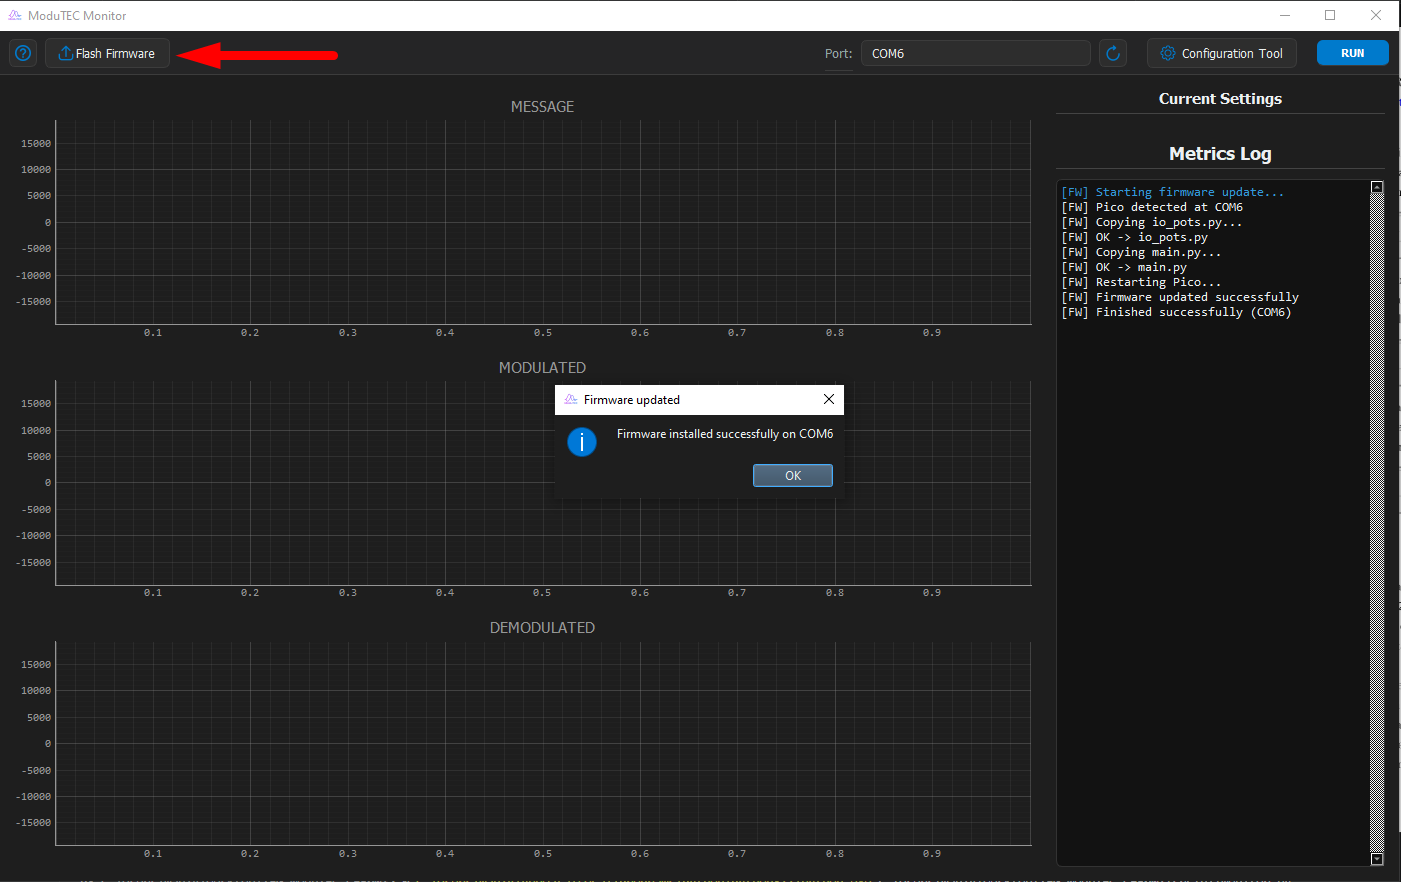
\includegraphics[width=1\textwidth]{../fig/firmware.png}
    \caption{Proceso de despliegue automático del firmware utilizando ModuTEC.}
    \label{fig:automatic_deployment}
\end{figure}

% ------------------------------------------------
\chapter{Uso de la Herramienta}
% ------------------------------------------------
\section{Detección de la Raspberry Pi Pico}

Antes de iniciar el monitoreo, la Raspberry Pi Pico debe encontrarse conectada mediante el cable USB y con el firmware previamente cargado. Una vez abierta la aplicación ModuTEC, se recomienda utilizar la opción \textit{Refresh Ports} para actualizar la lista de puertos seriales disponibles y detectar automáticamente el dispositivo conectado.

Al finalizar la búsqueda, el puerto asociado a la Raspberry Pi Pico aparecerá disponible dentro de la aplicación y podrá ser utilizado para establecer la comunicación con el sistema.

\begin{figure}[H]
\centering
% Captura de pantalla
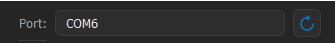
\includegraphics[width=0.6\textwidth]{../fig/refresh-ports.png}
\caption{Detección de puertos disponibles mediante la opción Refresh Ports.}
\end{figure}

\section{Configuración del sistema}

ModuTEC incorpora una herramienta de configuración denominada \textit{Config Tool}, la cual permite modificar los parámetros globales del sistema y generar automáticamente el archivo \texttt{config.json} utilizado por el firmware.

Desde esta interfaz es posible ajustar parámetros relacionados con la frecuencia de muestreo, tamaño de bloque, amplitud de las señales y rangos de operación de cada técnica implementada.

\begin{figure}[H]
\centering
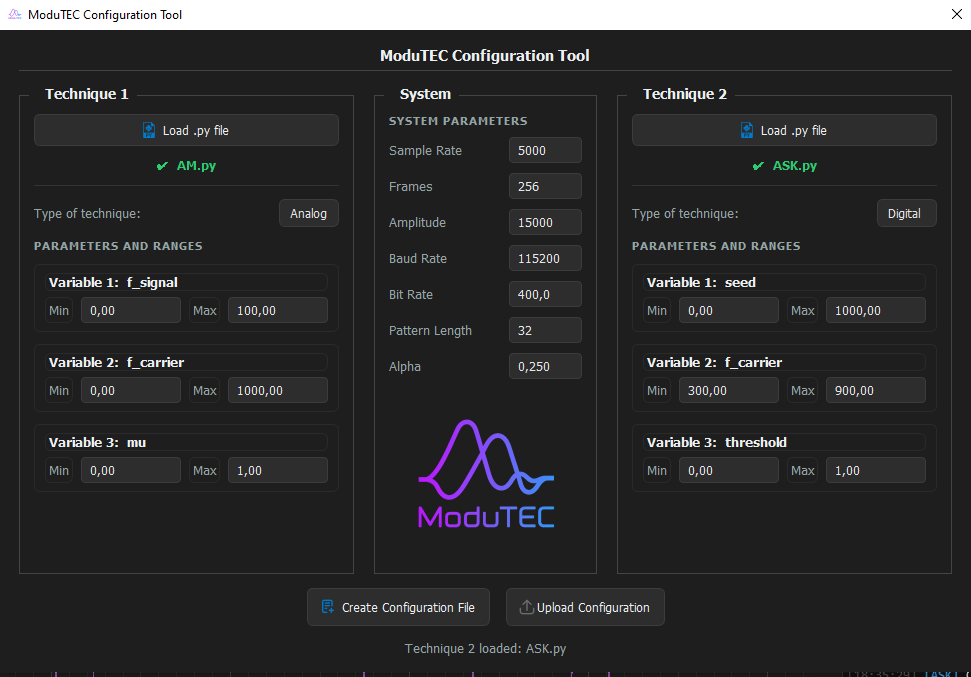
\includegraphics[width=0.85\textwidth]{../fig/config-tool.png}
\caption{Herramienta de configuración de ModuTEC.}
\end{figure}

Los parámetros globales disponibles se describen en la Tabla~\ref{tab:config_params}.

\begin{table}[H]
\centering
\caption{Parámetros globales configurables desde Config Tool.}
\label{tab:config_params}
\begin{tabularx}{\textwidth}{p{3cm}p{2cm}X}
\toprule
\textbf{Campo} & \textbf{Tipo} & \textbf{Descripción} \\
\midrule
\texttt{sample\_rate} & int &
Frecuencia de muestreo utilizada para generar y procesar las señales del sistema. \\

\texttt{frames} & int &
Cantidad de muestras procesadas y transmitidas en cada bloque de datos. \\

\texttt{amplitude} & int &
Amplitud máxima utilizada para escalar las señales antes de su transmisión. \\

\texttt{baud\_rate} & int &
Velocidad de comunicación serial utilizada entre la Raspberry Pi Pico y el monitor. \\

\texttt{bit\_rate} & float &
Tasa de bits empleada por las técnicas de modulación digital. \\

\texttt{pattern\_length} & int &
Longitud del patrón pseudoaleatorio utilizado para la generación de datos digitales de prueba. \\

\texttt{alpha} & float &
Coeficiente utilizado por los filtros digitales de demodulación basados en suavizado exponencial. \\
\bottomrule
\end{tabularx}
\end{table}

Adicionalmente, cada técnica posee adicionalmente tres parámetros específicos
asociados a los potenciómetros físicos del sistema. El rango de valores para
estos parámetros puede ser definido directamente dentro de la misma herramienta
de configuración. Una vez completada la configuración, el archivo \texttt{config.json}
puede generarse automáticamente y posteriormente puede cargarse directamente al
dispositivo utilizando la función de transferencia integrada dentro de la aplicación.

\section{Inicio del monitoreo}

Una vez transferida la configuración y conectado el dispositivo, el monitoreo puede
iniciarse mediante el botón \textit{Run}. Al establecerse la comunicación con la
Raspberry Pi Pico, la ventana principal comenzará a mostrar en tiempo real las señales
generadas por el sistema como se muestra en la Figura~\ref{fig:main_monitor}.

\begin{figure}[H]
\centering
\label{fig:main_monitor}
% Captura de pantalla
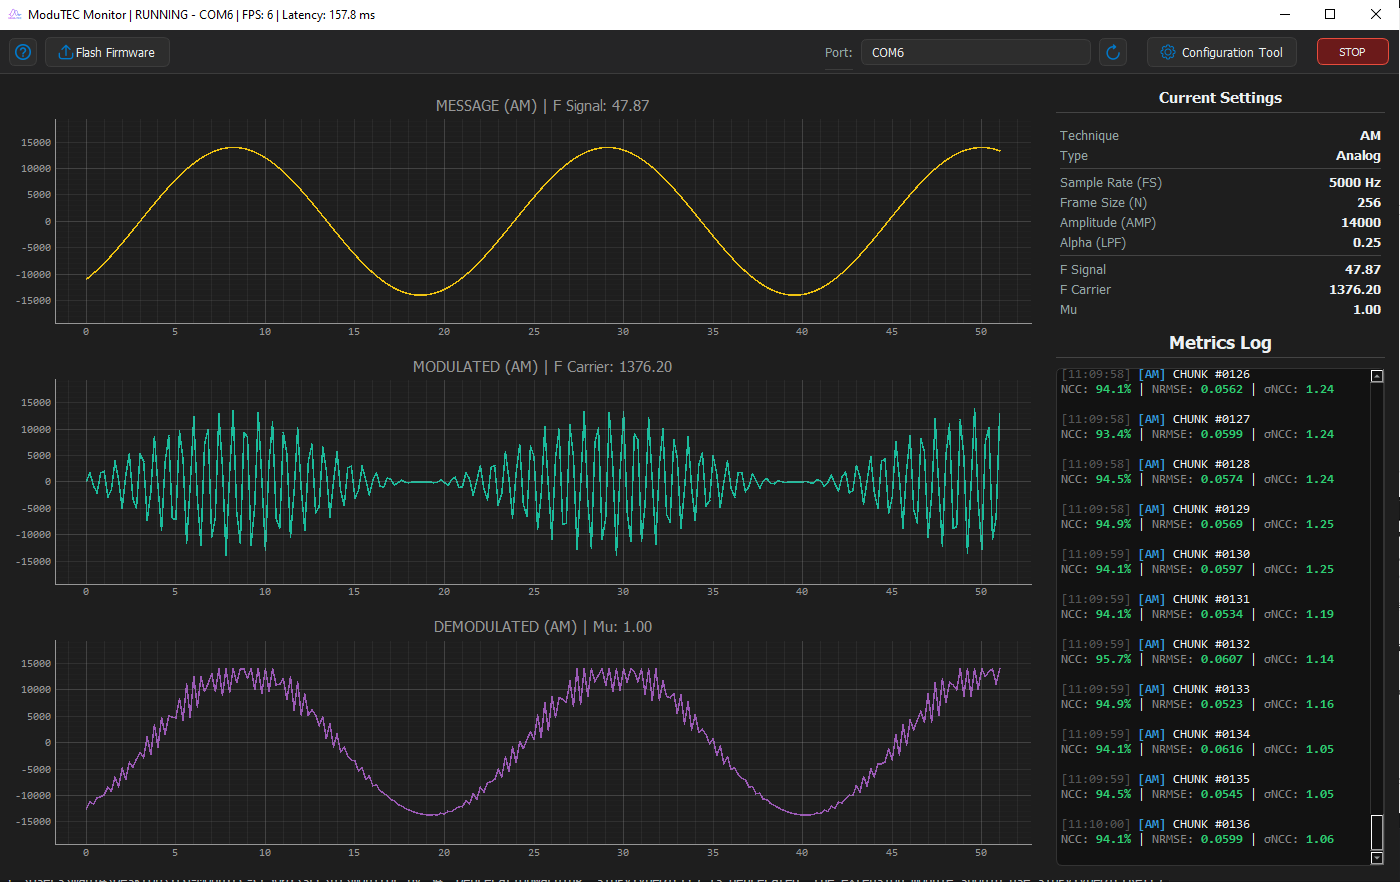
\includegraphics[width=0.69\textwidth]{../fig/main-monitor.png}
\caption{Ventana principal del monitor ModuTEC durante la ejecución.}
\end{figure}

\section{Selección de técnicas y ajuste de parámetros}

La técnica de modulación activa se selecciona mediante el interruptor físico conectado
a la Raspberry Pi Pico. Actualmente el sistema soporta 2 técnicas por ejecución, pueden
ser tanto analógicas como digitales, por defecto ModuTEC posee Modulación por Amplitud (AM)
y Modulación por Desplazamiento de Amplitud (ASK/OOK) precargadas, pero el usuario podrá
agregar nuevas técnicas siguiendo el procedimiento descrito más adelante.

Los parámetros específicos de cada técnica se ajustan mediante los tres potenciómetros
conectados al sistema. Cada potenciómetro controla un parámetro definido dentro de cada
técnica,permitiendo modificar su valor en tiempo real el cual es mostrado tambien desde 
la interfaz de ModuTEC.


% ------------------------------------------------
\chapter{Extensión de la Plataforma}
% ------------------------------------------------

\section{Creación de nuevas técnicas}

Para agregar una nueva técnica de modulación y demodulación a ModuTEC, únicamente se requieren dos pasos:

\begin{enumerate}
\item Crear un archivo Python que implemente la técnica siguiendo la estructura estándar proporcionada en el Apéndice~\ref{ap:template}.
\item Registrar la técnica mediante la herramienta \textit{Config Tool}, definiendo sus parámetros y rangos de operación.
\end{enumerate}

Una vez completados estos pasos, la configuración generada puede transferirse al microcontrolador utilizando las herramientas integradas de ModuTEC, quedando la nueva técnica disponible para su ejecución.

\section{Elementos obligatorios del template}

Toda nueva técnica debe ser creada en un archivo de Python con el nombre de la técnica (p.\,ej.\ \texttt{PSK.py}) y debe incluir los siguientes elementos:

\begin{itemize}

\item \textbf{\texttt{PARAM\_ORDER}}: lista que define el nombre y orden de los parámetros asociados a los tres potenciómetros físicos.

\item \textbf{\texttt{State}}: estructura utilizada para almacenar variables que deben mantenerse entre bloques de procesamiento, como fases acumuladas, estados de filtros o contadores internos.

\item \textbf{\texttt{compute\_frame()}}: función principal encargada de procesar la señal mensaje, la señal modulada y la señal demodulada para cada bloque de muestras.

\end{itemize}

Estos elementos constituyen la interfaz mínima requerida por el firmware para cargar y ejecutar dinámicamente cualquier técnica registrada. Una vez respetada esta estructura, la lógica interna de modulación y demodulación puede implementarse libremente según las características de la técnica desarrollada. Por ejemplo, una técnica analógica puede requerir almacenar fases de portadora y estados de filtros, mientras que una técnica digital podría necesitar registros de símbolos, contadores de bits o generadores pseudoaleatorios. Como referencia, el Apéndice~\ref{ap:template} incluye un archivo base que puede utilizarse como punto de partida para la implementación de nuevas técnicas compatibles con ModuTEC.

% =====================================================
% APENDICES
% =====================================================
\appendix
\chapter{Plantilla de código para nuevas técnicas}
\label{ap:template}
% ------------------------------------------------

A continuación se presenta el template completo que debe utilizarse como punto de partida
para implementar cualquier nueva técnica en ModuTEC. Las secciones marcadas como
\texttt{\# Ejemplo:} deben ser reemplazadas con la lógica específica de la técnica; los
comentarios de estructura deben mantenerse para facilitar la revisión y el mantenimiento.

\begin{lstlisting}[language=Python, caption={TECHNIQUE\_NAME.py - Template}]
import math
import struct

# -- Definicion explicita del orden de parametros --
PARAM_ORDER = ["param_1", "param_2", "param_3"]


def _clamp(x, lo, hi):
    return lo if x < lo else hi if x > hi else x


class State:
    """
    Estado de TECHNIQUE_NAME.
    Agregar aqui todas las variables que necesitan persistir
    entre frames.
    """

    __slots__ = (
        # Ejemplo: "phase_c", "lpf_y", etc.
    )

    def __init__(self):
        pass
        # Ejemplo:
        # self.phase_c = 0.0
        # self.lpf_y   = 0.0


def compute_frame(state, params, sys_cfg):
    """
    Interfaz estandar ModuTEC.

    Parametros esperados en params (deben coincidir con
    config.json):
        - param_1 : descripcion y unidades
        - param_2 : descripcion y unidades
        - param_3 : descripcion y unidades

    Retorna:
        payload_m   : bytearray int16 -- senal mensaje
        payload_mod : bytearray int16 -- senal modulada
        payload_dem : bytearray int16 -- senal demodulada
    """

    # -- Extraer parametros del sistema ---------------------
    FS    = sys_cfg["fs"]
    N     = sys_cfg["n"]
    AMP   = sys_cfg["amp"]
    alpha = sys_cfg["alpha"]
    # Tecnicas digitales pueden necesitar ademas:
    # bit_rate    = sys_cfg["bit_rate"]
    # pattern_len = sys_cfg["pattern_len"]

    # -- Extraer parametros de la tecnica -------------------
    param_1 = params["param_1"]
    param_2 = params["param_2"]
    param_3 = params["param_3"]

    # -- Inicializar buffers de salida ----------------------
    payload_m   = bytearray(2 * N)
    payload_mod = bytearray(2 * N)
    payload_dem = bytearray(2 * N)

    # -- Restaurar estado -----------------------------------
    # Ejemplo:
    # phase_c = state.phase_c
    # lpf_y   = state.lpf_y

    # -- Loop de generacion muestra a muestra ---------------
    for i in range(N):

        # Calcular senales (rango normalizado -1..1)
        msg = 0.0  # senal mensaje
        s   = 0.0  # senal modulada
        dem = 0.0  # senal demodulada

        # Escribir muestras en buffers
        struct.pack_into("<h", payload_m,   2 * i, int(AMP * msg))
        struct.pack_into("<h", payload_mod, 2 * i, int(AMP * s))
        struct.pack_into("<h", payload_dem, 2 * i, int(AMP * dem))

        # Actualizar variables de fase u otras internas del loop

    # -- Guardar estado para el proximo frame ---------------
    # Ejemplo:
    # state.phase_c = phase_c
    # state.lpf_y   = lpf_y

    return payload_m, payload_mod, payload_dem
\end{lstlisting}

\end{document}